
\textit{Results from this chapter are preliminary and have not been reviewed yet by the LIGO Scientific Collaboration.}
%\newline

        \section{Directed TwoSpect}
        \label{directed}

TwoSpect performed aptly in Chapter~\ref{chap5}'s Mock Data Challenge, which warrants using the program to analyze the best existing GW data.
At the time of writing, the best consistent stretch of data remains Science Run 6 (S6) taken from 2009 July 09 to 2010 October 20 by LIGO Hanford Observatory (LHO) and LIGO Livingston Observatory (LLO).
Advanced LIGO (aLIGO) commissioning is already surpassing the sensitivity of S6 for short periods of time.
While early LIGO continuous wave (CW) searches used short science runs such as S2~\cite{AbbottScoX12007}, aLIGO data duration is for now too short for an analysis competitive with present upper limits, in particular the 2011 Radiometer~\cite{AbadieStoch2011} S5 high frequency results and 2014 TwoSpect~\cite{GoetzTwoSpectResults2014} S6 low frequency results.
The increased sensitivity anticipated from aLIGO Observing Run 1 (O1), which is planned to last several months in summer 2015, could yield interesting results, and the year-length O3 is planned before the end of the decade.
Scorpius X-1 broadband upper limits from S6 are the direction of this chapter.

            %TwoSpect improvements myself (to do).

            \subsection{Targeted, directed and all-sky search sensitivity}
            \label{tradeoffs}

Several approaches exist toward a search from GW from known objects such as Scorpius X-1.
When seeking continuous GW, these methods are classified as all-sky, directed, or targeted, in order of increasing focus of the search.
More focused searches make sense as more prior information is known, such as sky location, neutron star frequency and binary system orbital parameters.
Additional information lets some CW searches refine, for instance, their template models of GW signals.If the search is designed for minimal information, in particular if sky location is unknown, it is generally called an \textit{all-sky search}.
Some information -- such as a low-uncertainty sky-location, much less than a square radian -- helps what are called \textit{directed searches} gain sensitivity.
Sources with comprehensively-documented parameters, such as rotation frequency and spindown rate, lend themselves to \textit{targeted searches} that search over a very narrow range of parameters, \textit{e.g.,} putative GW phase, that cannot be deduced with other instruments.

TwoSpect was designed~\cite{GoetzThesis,GoetzTwoSpectMethods2011} as an all-sky search for unknown neutron stars.
The voluminous parameter space of that search, as described in Chapter~\ref{chap5}, prompted tradeoffs in sensitivity vs computational cost, in particular the limitation of test statistic calculation to only those outlier candidates that survived an incoherent harmonic sum stage. 
For objects with constrained sky location and NS parameters, thorough calculations of the $R$ test statistic become feasible.

For Scorpius X-1, many parameters are known (updated ephemerides were calculated in 2014 by Galloway~\cite{Galloway2014}), but critically, rotation frequency is not.
Sky location is known, and the period is $0.7873114 \pm 0.0000005$ days, \textit{i.e.,} $68023.70 \pm 0.04$ s with 1-$\sigma$ uncertainty\footnote{Access to a preliminary ephemeris in the MDC led us to use $P = 68023.8259 s$ in for searches in the MDC and S6; MDC simulations justify assuming that this variation has negligible impact on TwoSpect, which would only be able to discriminate between different periods around $68023 s$ at a resolution of about $40 s$ or greater, depending on Fourier transform coherence time.}.
The projected semimajor axis, $a \sin i$, is $1.44 \pm 0.18 s$ with 1-$\sigma$ uncertainty\footnote{Orbital parameters interpreted in correspondence between C. Messenger and D. Galloway.}.
Rotation frequency uncertainty drives the cost of the search.
While the Chakrabarty speed limit~\cite{Chakrabarty2003} and neutron star breakup limit limit $2\nu$, the GW emission frequency of an NS quadrupole, to $\mathcal{O}(2\textup{ to }3)$ kHz, the dominant high frequency limit $f_h$ is driven as much by the noise floor of the LIGO detectors.
This noise floor increases proportionally to the square root of frequency and at 2 kHz is an order of magnitude worse than its most sensitive, about $2\times10^{-23}$ in dimensionless strain between 150 and 200 Hz.
Photon shot noise, that is, quantum vacuum fluctuations are the limiting noise source at those frequencies.
The low frequency limit, $f_l$, is also driven by the noise floor of the detector, which becomes contaminated by seismic noise below about 40 Hz.

A search for Scorpius X-1 in S6 data should thus take place between about 40 and 2000 Hz. 
TwoSpect requires shortened Short Fourier Transforms (SFTs)~\cite{GoetzTwoSpectMethods2011} to fully capture the spectral power if a GW source has a high frequency or $a \sin i$. 
This suggests dividing the main search: 40 to 360 Hz can be searched in 840 s coherence time SFTs and 360 to 2040 Hz in 360 s coherence time SFTs.
These sets constitute the primary search.
Although MDC and simulation experience suggests spectral power is lost only slowly as GW frequency exceeds optimal coherence time, we have also prepared 260 to 360 Hz SFTs with 360 s coherence time and 1400 to 2040 Hz SFTs with 300 s coherence time; these are most useful for high $a \sin i$ signal models.
These additional sets constitute the `overlap' search.
Calculating the number of templates in the primary search (the overlap search is smaller because of shorter coherence times) over these frequencies and $\pm 3 \sigma_{a \sin i}$, if analyzed in 0.1 Hz computational bands\footnote{0.1 Hz computational bands fit efficiently on cluster memory in under 2 GB of RAM; for convenience, templates are (redundantly) tested at both the lower \& upper bounds of the 0.1 Hz.} using Equation~\ref{N_template_simple},

\begin{equation}
N_\textup{template} = 2 (840.1)\left[1+ \frac{3360\pi}{68023.8} 400.1 \right](320) + 2 (360.1)\left[1+ \frac{1440\pi}{68023.8}2400.1\right](1680),
\label{S6_N_templates}
\end{equation}

\noindent or $3.392\times 10^7$ templates in 840 s SFTs and $1.9434\times 10^8$ templates in 360 s SFTs, per interferometer.
Searching both LHO's H1 interferometer and LLO's L1 interferometer, the grand total is $4.5652\times10^8$ templates.

Each of these templates takes between 0.3 and 3 s to run on late 2000s to early 2010s CPUs, depending on vector extensions (such as SSE) and clock speed.
Given approximately two thousand cores at a cluster such as the LIGO Data Grid at the California Institute of Technology and the LIGO observatories or Atlas at the Albert Einstein Institute in Hannover, Germany, a fully templated TwoSpect search for Scorpius X-1 in S6 data can be completed in roughly a month.
This has been carried out by the author and is the subject of the remainder of this chapter.
Because of the enhanced sensitivity and wider frequency range of the directed search, this analysis can improve on the TwoSpect all-sky limits by Goetz~\cite{GoetzTwoSpectResults2014} while consuming comparable computational resources (albeit for a single, promising source).

             %   Targeted (known object) vs directed (region)vs all-sky (everything).

            \subsection{Enhancements enabled by directed searching}
            \label{directed_enhancements}

Directed TwoSpect as used for the search in this chapter closely resembles the all-sky TwoSpect pipeline, except for post-processing. 
The post-processing is discussed below.
The bulk of the processing,skipping the incoherent harmonic sum stage that reduces the number of templates search, involves generating the test statistic, $R$, for each point in a rectangular grid spaced at $1/(2T_\textup{coh})$ in frequency and $1/(4T_\textup{coh})$ in $a \sin i$, which keeps mismatch between putative signal and template to within 0.2 of the peak $R$ value~\cite{GoetzTwoSpectMethods2011}.
Since sky location and period are fixed, the search is two-dimensional on the $f$ and $a \sin i$. 
Because the detector frame realization of $a \sin i$ is as a frequency modulation, $df$, this search space can be describes as the `$df$ vs $f$' plane.
Each pixel in the `$df$ vs $f$' plane has an $h_0$ and $\log_{10} p$-value associated with its $R$ statistic, as noted in Chapter~\ref{chap5}.
The $h_0$ is proportional to $R^{1/4}$; $\log_{10} p$ is more complicated but loosely scales with $R$ in Gaussian noise and has been calibrated into an accurate, single-template $p$-value using Davies' method.
Our search uses $\mathcal{O}(10^8)$ templates, not single-templates nor a few, distant-and-uncorrelated templates as in the all-sky search.
Thus the directed search necessitates enhancements to post-processing.

In the near future, enhancements enabled by the directed search will be possible.
Sensitivity from full templating is the first step.
The next steps can involve a search over orbital phase and polarization with additional computation steps and templating techniques.
Before these extra dimensions, however, the author has had to validate new approaches to analyzing this dense 2D parameter space.


             %   Modifications for directed search.

        \section{Quantifying directedness: sensitivity studies in real data}
        \label{quant_directed}


            %Quantify how good the improvements are in directed TwoSpect. 

            Cite Feldman-Cousins confidence intervals paper~\cite{FeldmanCousins1998}.

            Cite Ethan's thesis~\cite{RomeroThesis} and our paper, maybe by using generation functions to make better TwoSpect statistics.

      %\section{Real S6 data: statistics}

        \subsection{Real S6 data: detection efficiency}

\begin{figure}
\begin{center}
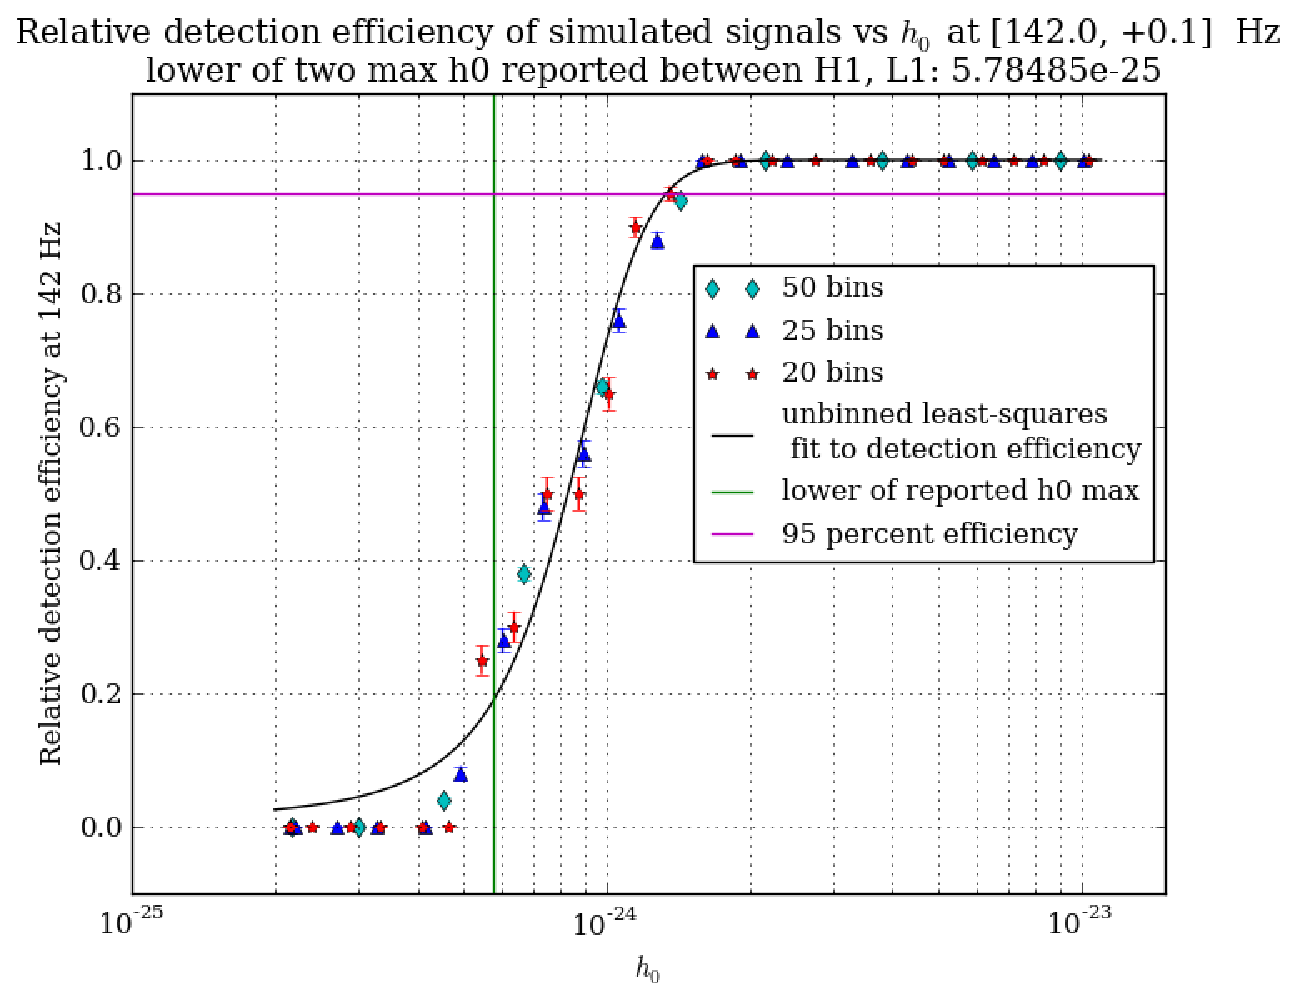
\includegraphics[width=0.4\paperwidth,height=0.2\paperheight]{plots/detectionEfficiencyh0-142-0Hz.eps}
\caption{Detection efficiency of 500 injections (each at H1, L1) into
S6 data at 142 Hz, given threshold log10p = -7.75}
\end{center}
\end{figure}

        \subsection{Real S6 data: $h_0$ recovered vs injected}

\begin{figure}
\begin{center}
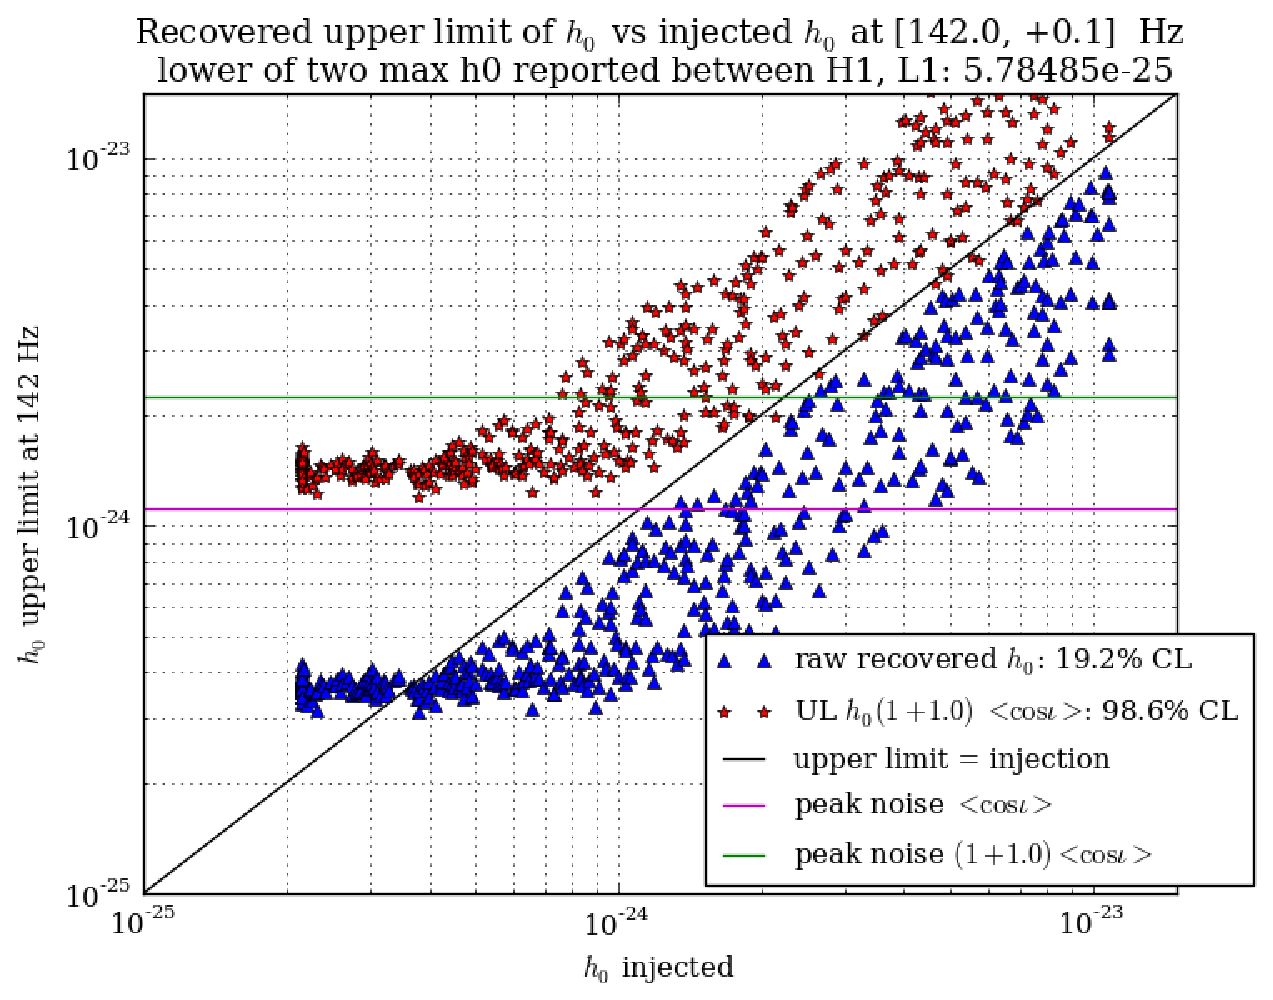
\includegraphics[width=0.4\paperwidth,height=0.2\paperheight]{plots/h0UL-vs-h0injected-142-0Hz.eps}
\caption{
Raw $h_0$ \& tentative 95\% confidence UL $>2\times10^{-24}$; 500 injections
into S6 data at 142 Hz (injections also done at 162, 222 Hz)}
\end{center}
\end{figure}

See Appendix~\ref{appendix2} for further injection studies.



%\section{S6: Scorpius X-1}

        \section{Scorpius X-1 search using Directed TwoSpect in S6}
        \label{directed_results}
 
            %Preliminary results of a directed search (possibly simulation-only).

            %We have a great deal of material here already, just need to pull from figures and commentary from the Sco X-1 wiki. Keith recommends paralleling the Sco X-1 paper.



\subsection{S6: Scorpius X-1 search plan}

\textbf{2 kHz, $\pm 3 \sigma_{a \sin i}$ search over all S6 data from H1 \& L1}
\begin{itemize}
\item Analyze 40 to 360 Hz with 840 s SFTs,
\item Analyze 360 to 2040 Hz with 360 s SFTs,\\
(to prevent spectral leakage)
\item Now planned: overlapping bands to verify
\item Search over 300+1100 Hz = 1.4 kHz complete on H1
\item Search over 300+1700 Hz = 2.0 kHz complete on L1
\end{itemize}


\subsection{S6: Scorpius X-1 heatmaps}

\begin{figure}
\begin{center}
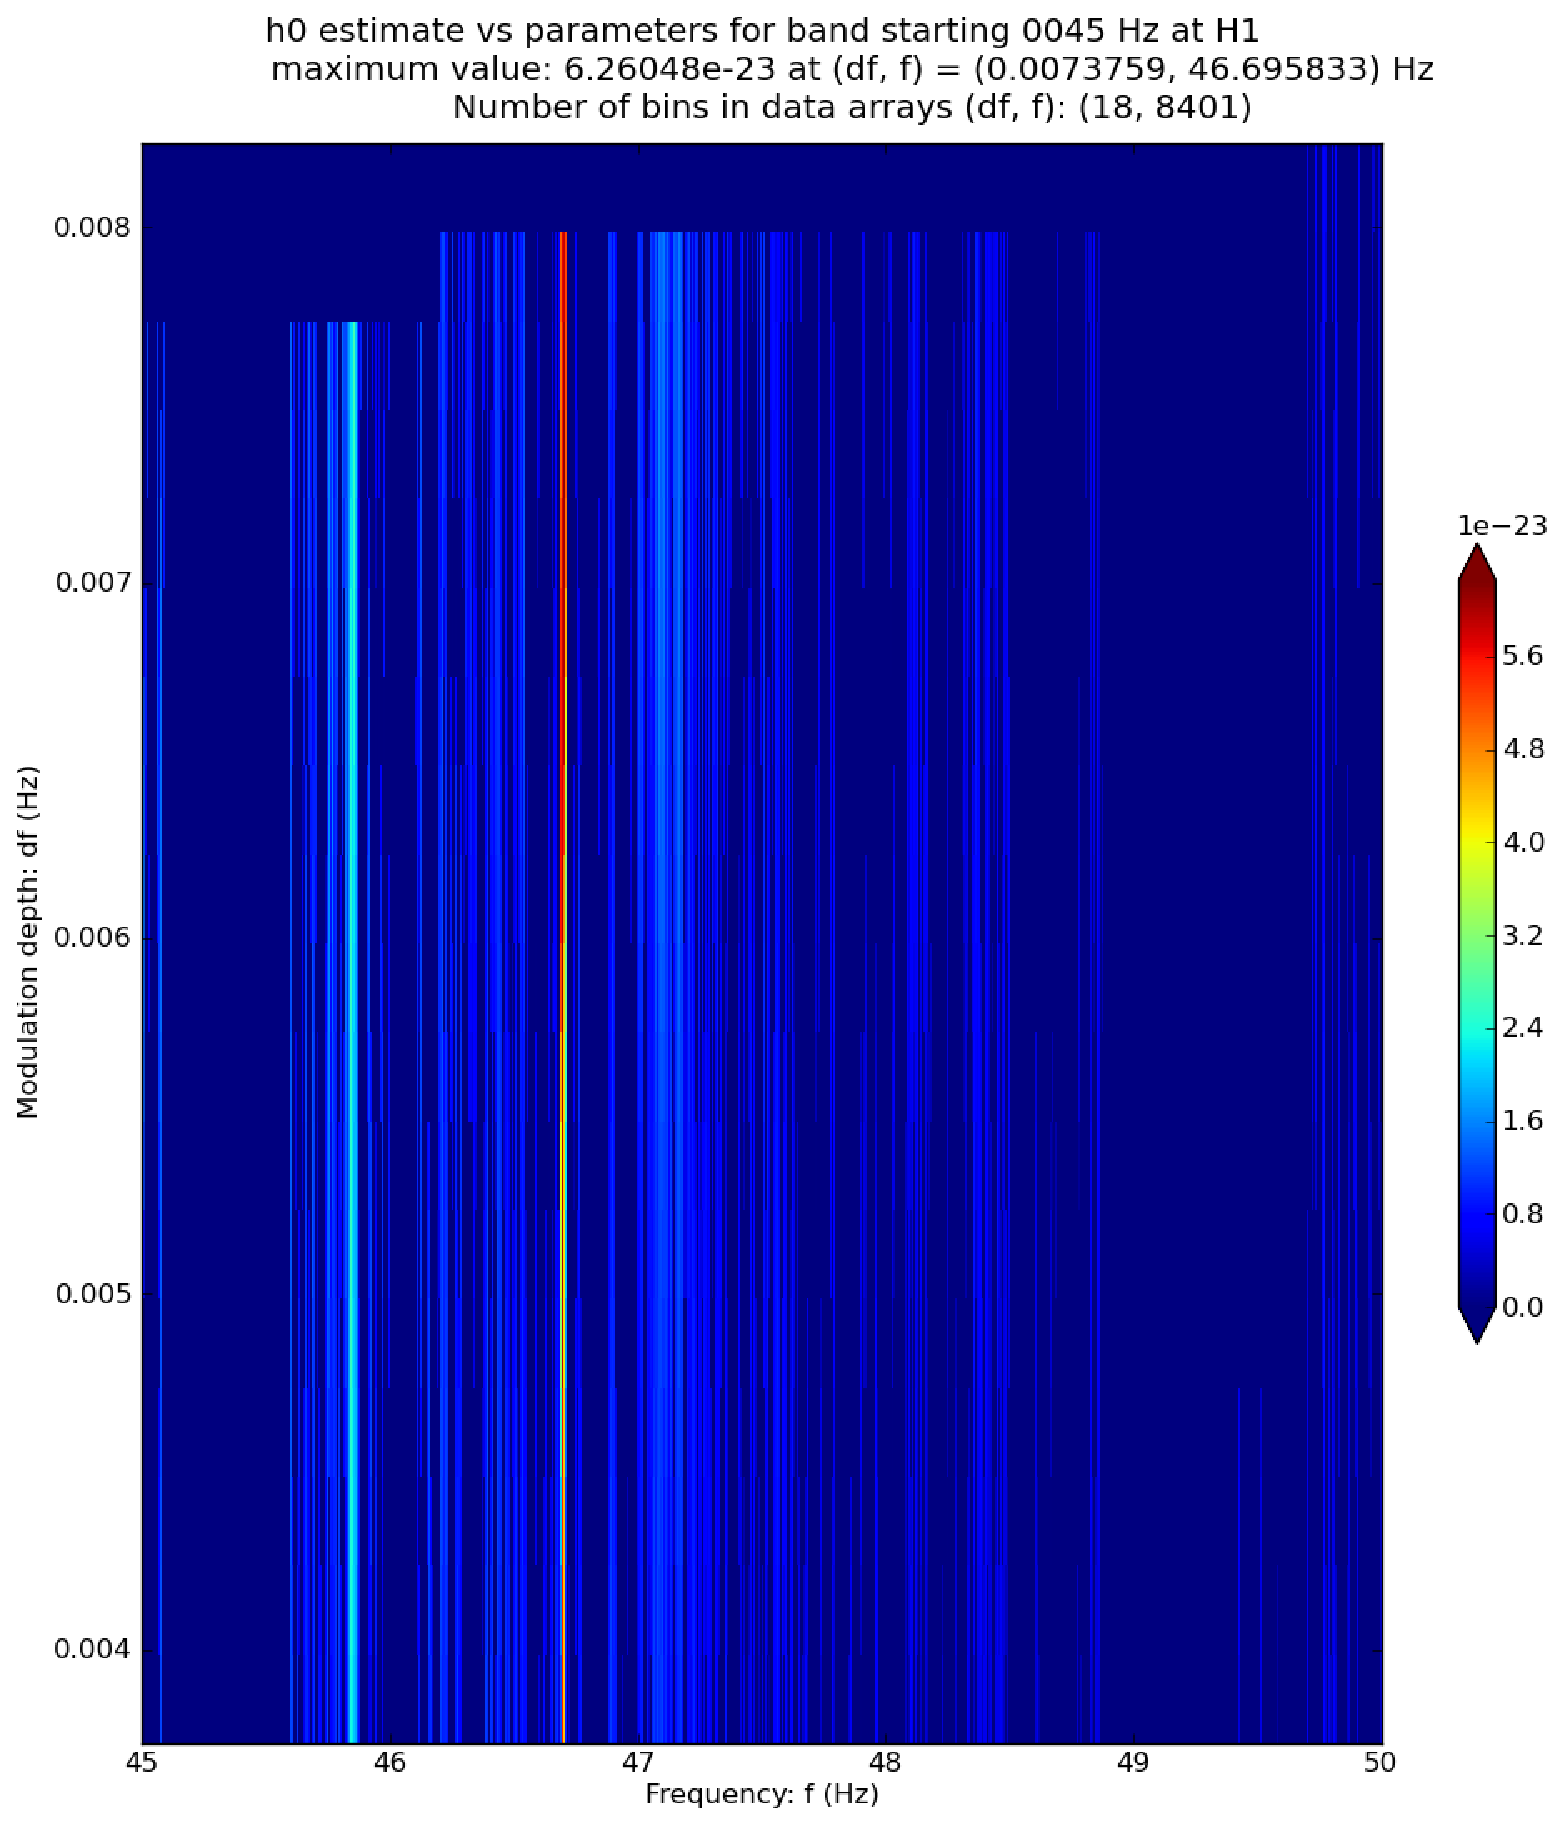
\includegraphics[width=0.4\paperwidth,height=0.2\paperheight]{plots/DFvsFresultsh0-H1_pulsar-0045.eps}
\caption{
S6 $h_0$ heatmap shows real data features, such as 46.7 Hz cal line}
\end{center}
\end{figure}

\subsection{S6: Scorpius X-1 upper limits, random polarization}

\begin{figure}
\begin{center}
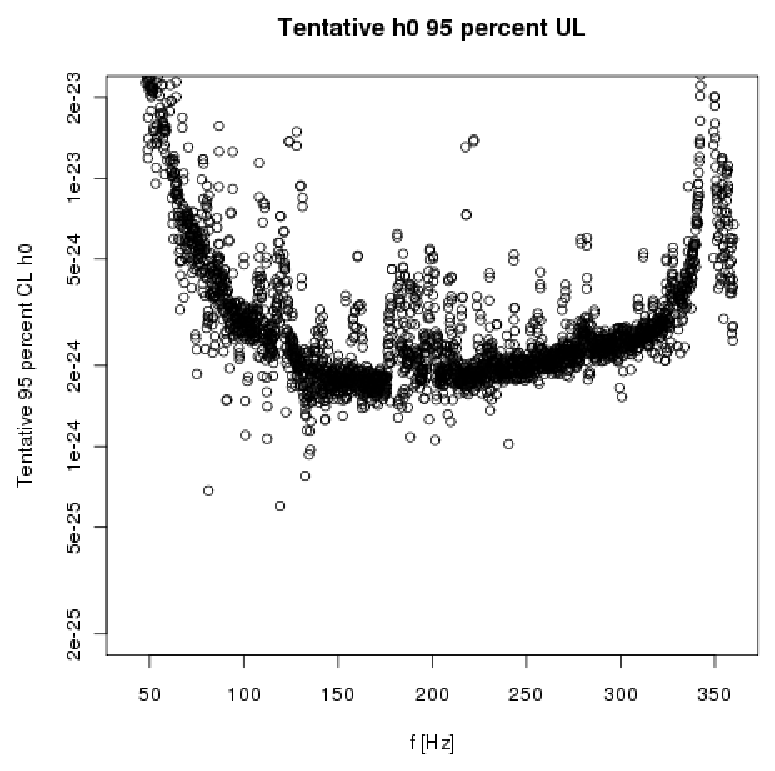
\includegraphics[width=0.4\paperwidth,height=0.2\paperheight]{plots/h0FullUL95logGuess-H1.eps}
\caption{
H1: loudest $h_0 \times \left( 1 + 0.8 \right) \times \left[\cos \iota \textup{ factor}\right]$ in 0.1 Hz bands}
\end{center}
\end{figure}

\begin{figure}
\begin{center}
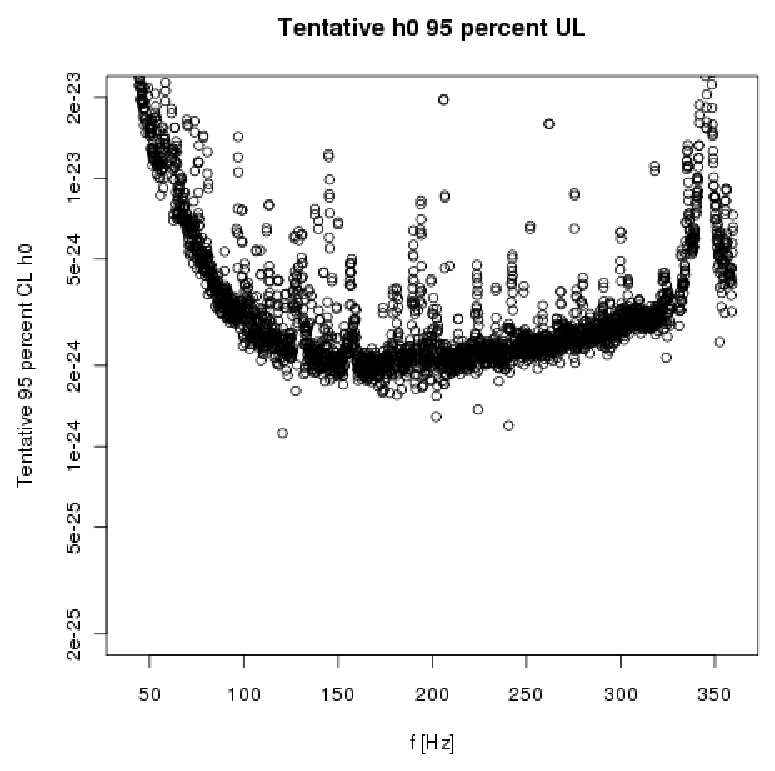
\includegraphics[width=0.4\paperwidth,height=0.2\paperheight]{plots/h0FullUL95logGuess-L1.eps}
\caption{
L1: loudest $h_0 \times \left( 1 + 0.8 \right) \times \left[\cos \iota \textup{ factor}\right]$ in 0.1 Hz bands}
\end{center}
\end{figure}

\begin{figure}
\begin{center}
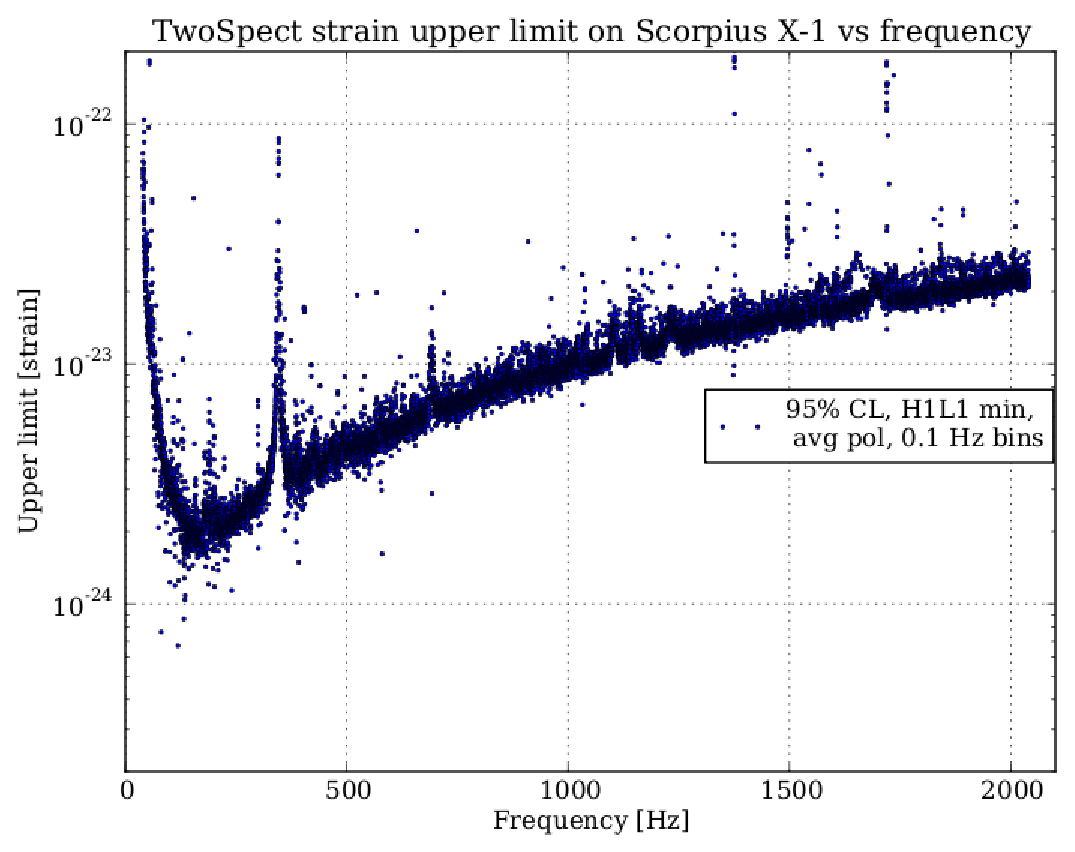
\includegraphics[width=0.8\paperwidth,height=0.4\paperheight]{plots/ScoX1ULs.eps}
\caption{
Joint upper limits for Scorpius X-1, using a confidence interval given by reported $h_0 \times \left( 1 + 1.0 \right) \times \left[\cos\iota \textup{ factor}\right]$ in 0.1 Hz bands. 
This spectrum covers 40 to 2040 Hz using the lower upper limit from either interferomer (H1 or L1) when both yielded data. 
A total of 28.8 Hz were in bands that yielded no real upper limit (because the quarter root of the test statistic was imaginary) in either interferometer, generally due to excessive noise in that band.
Bands were left-closed and right open, e.g., $\left[ 40.0,40.1\right), \left[ 40.1,40.2\right)\ldots \left[2039.9,2040.0\right)$.
}
\end{center}
\end{figure}

\subsection{S6: Scorpius X-1 outliers}

\begin{table}
\begin{center}
\begin{tabular}{r r l}
Outlier Number & Frequency (Hz) & Explanation \\
\hline
1 & 42.00 & \\
2 & 64.00 & \\
3 & 108.10 & \\
4 & 108.85 & \\
5 & 109.50 & \\
6 & 111.02 & \\
7 & 128.00 & \\
8 & 139.52 & \\
9 & 154.04 & \\
10 & 156.82 & \\
11 & 157.99 & \\
12 & 158.36 & \\
13 & 158.87 & \\
14 & 190.86 & \\
15 & 192.54 & Injected pulsar 8? \\
16 & 200.53 & \\
17 & 200.60 & \\
18 & 209.21 & \\
19 & 209.28 & \\
20 & 223.66 & \\
21 & 256.02 & \\
22 & 268.13 & \\
\end{tabular}
\caption{List of Scorpius X-1 outliers in the search of S6 data. This list covers 40 to 360 Hz.}
\label{ScoX1S6outlierTable}
\end{center}
\end{table}

Table~\ref{ScoX1S6outlierTable} presents a list of outliers present in both intereferometers.

\section{XTE J1751-305 search using Directed TwoSpect in S6}

\subsection{S6: XTE J1751-305 background}

Discovered by Markwardt et al in 2002~\cite{Markwardt2002}.

\textbf{XTE with shortest period, 42 minutes}\\
(P $\approx$$ $ 2545.3 s, $a \sin i$ $\approx0.010\pm0.003$s):\\
Search very fast ($< 10^5$ templates), promising target\\
\emph{although} estimated $d > 7$ kpc near galactic center
\\
$\textup{}$

\textbf{$\nu_0$}: 435.31799 Hz\\
\textbf{$r$-mode}: (2-0.5727597)*(435.31799 Hz) = 621.3034 Hz\\
$\textup{}$

\begin{description}
\item[{Searched frequencies}] [434.5,436.5] \& [620.5,622.5] Hz
\item{{Searching}} [869.5, 871.5]
\end{description}
$\rightarrow$ TwoSpect analysis, heatmaps done on $\nu_0$, $r$-mode\\
$\rightarrow$ Upper limits will be made

%\section{S6: XTE J1751-305}
\subsection{S6: XTE J1751-305 heatmaps}

\begin{figure}
\begin{center}
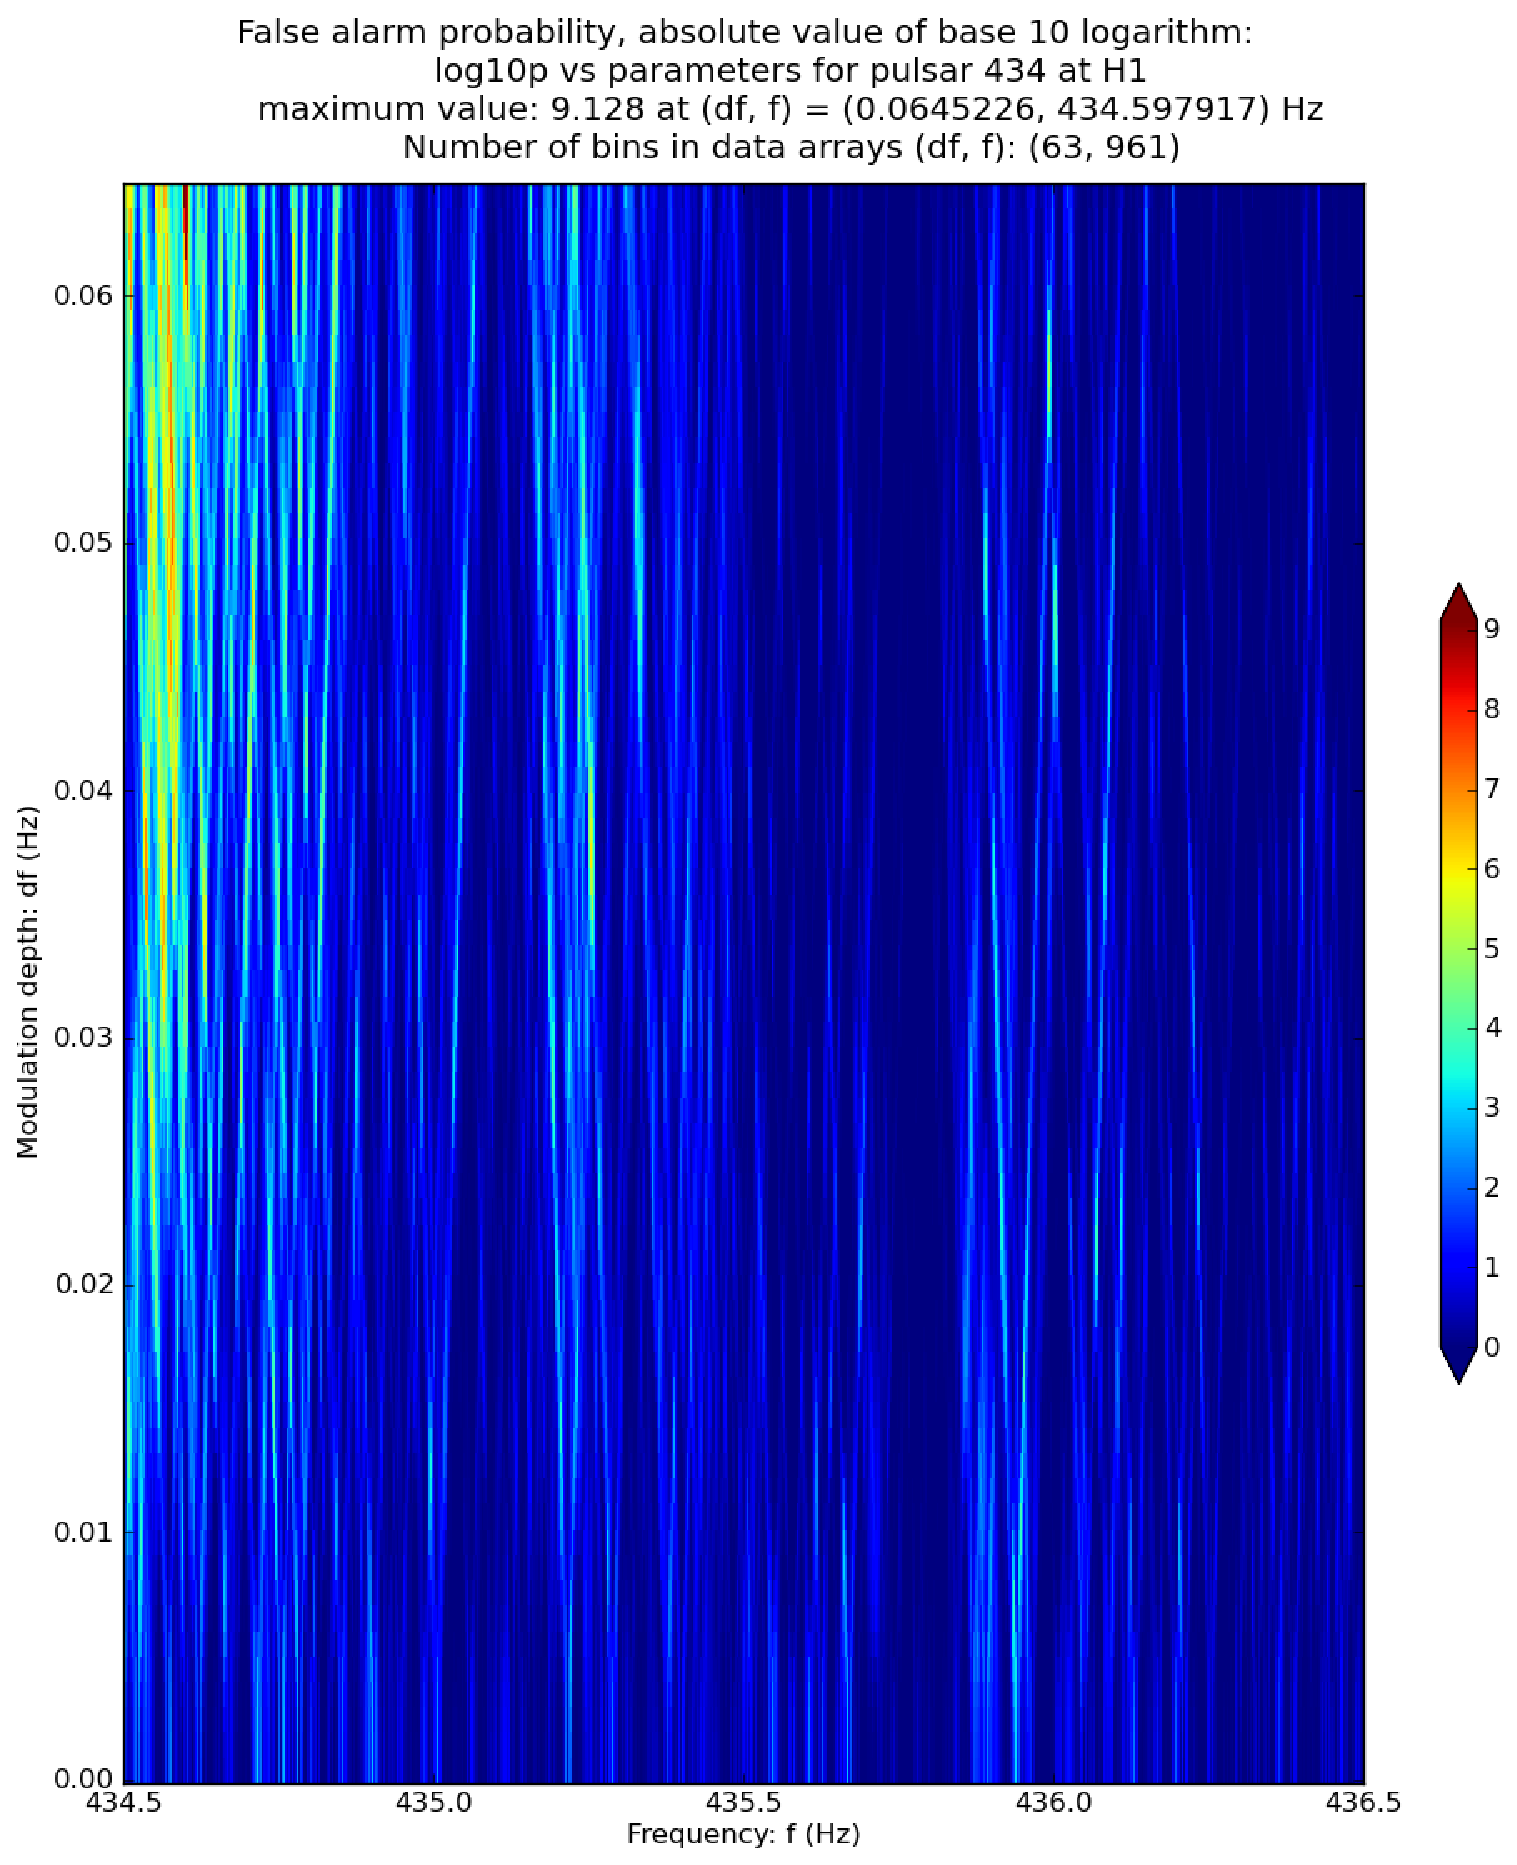
\includegraphics[width=0.4\paperwidth,height=0.2\paperheight]{plots/DFvsFresultsProb-H1_pulsar-434.eps}
\caption{
Quick look at J1751-305, H1 log10p, 435 Hz $\nu_0$}
\end{center}
\end{figure}


\begin{figure}
\begin{center}
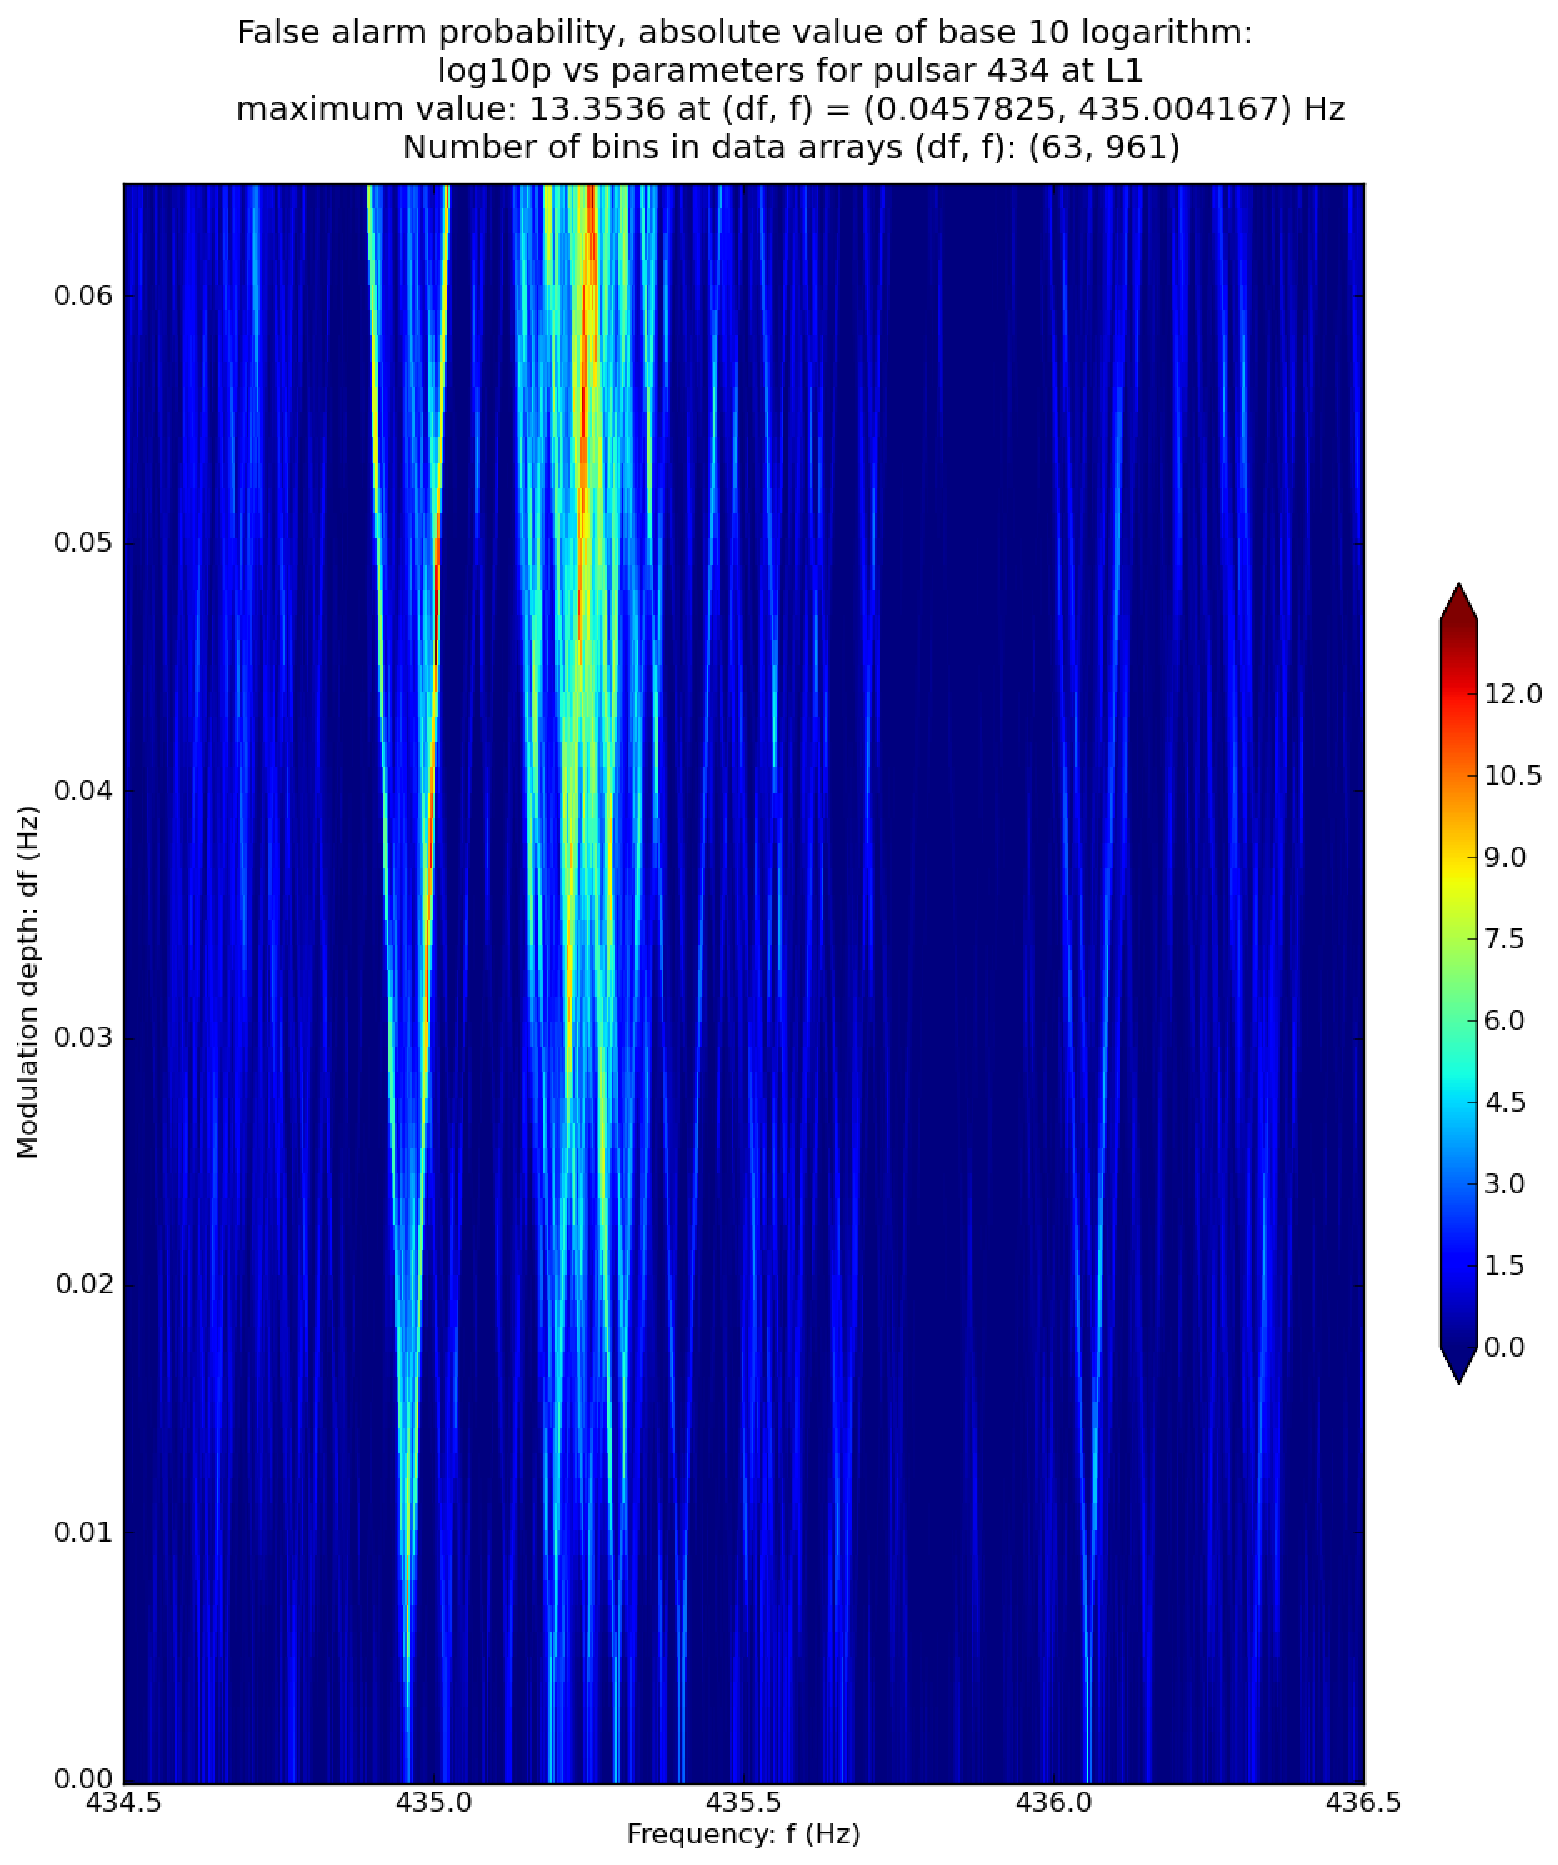
\includegraphics[width=0.4\paperwidth,height=0.2\paperheight]{plots/DFvsFresultsProb-L1_pulsar-434.eps}
\caption{
Quick look at J1751-305, L1 log10p, 435 Hz $\nu_0$}
\end{center}
\end{figure}


\begin{figure}
\begin{center}
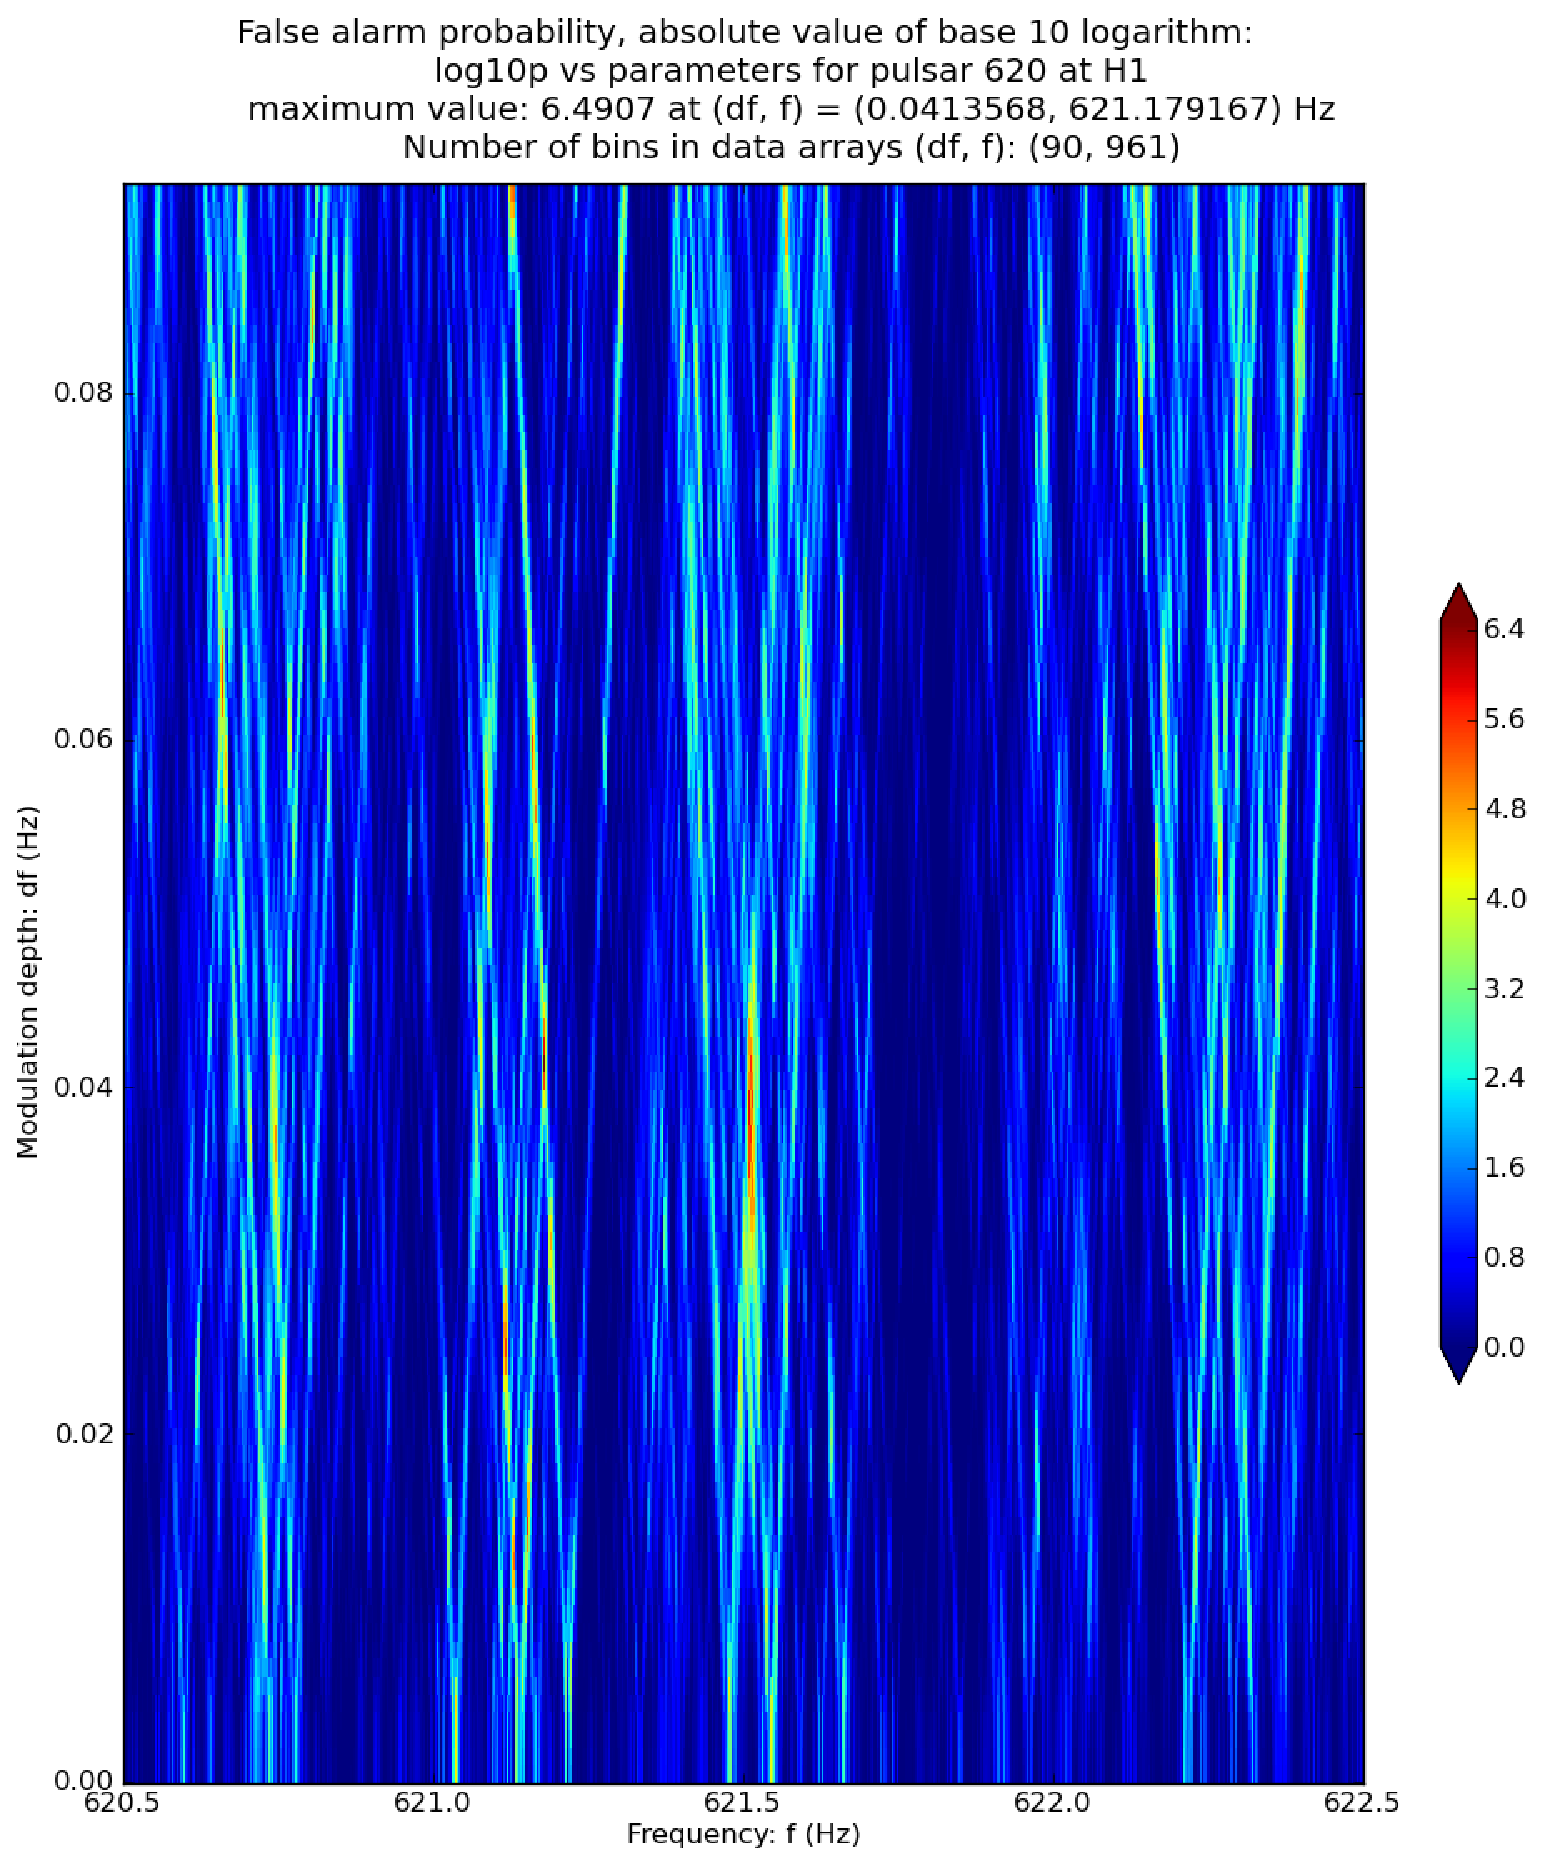
\includegraphics[width=0.4\paperwidth,height=0.2\paperheight]{plots/DFvsFresultsProb-H1_pulsar-620.eps}
\caption{
Quick look at J1751-305, H1 log10p, 621 Hz $r$-mode}
\end{center}
\end{figure}


\begin{figure}
\begin{center}
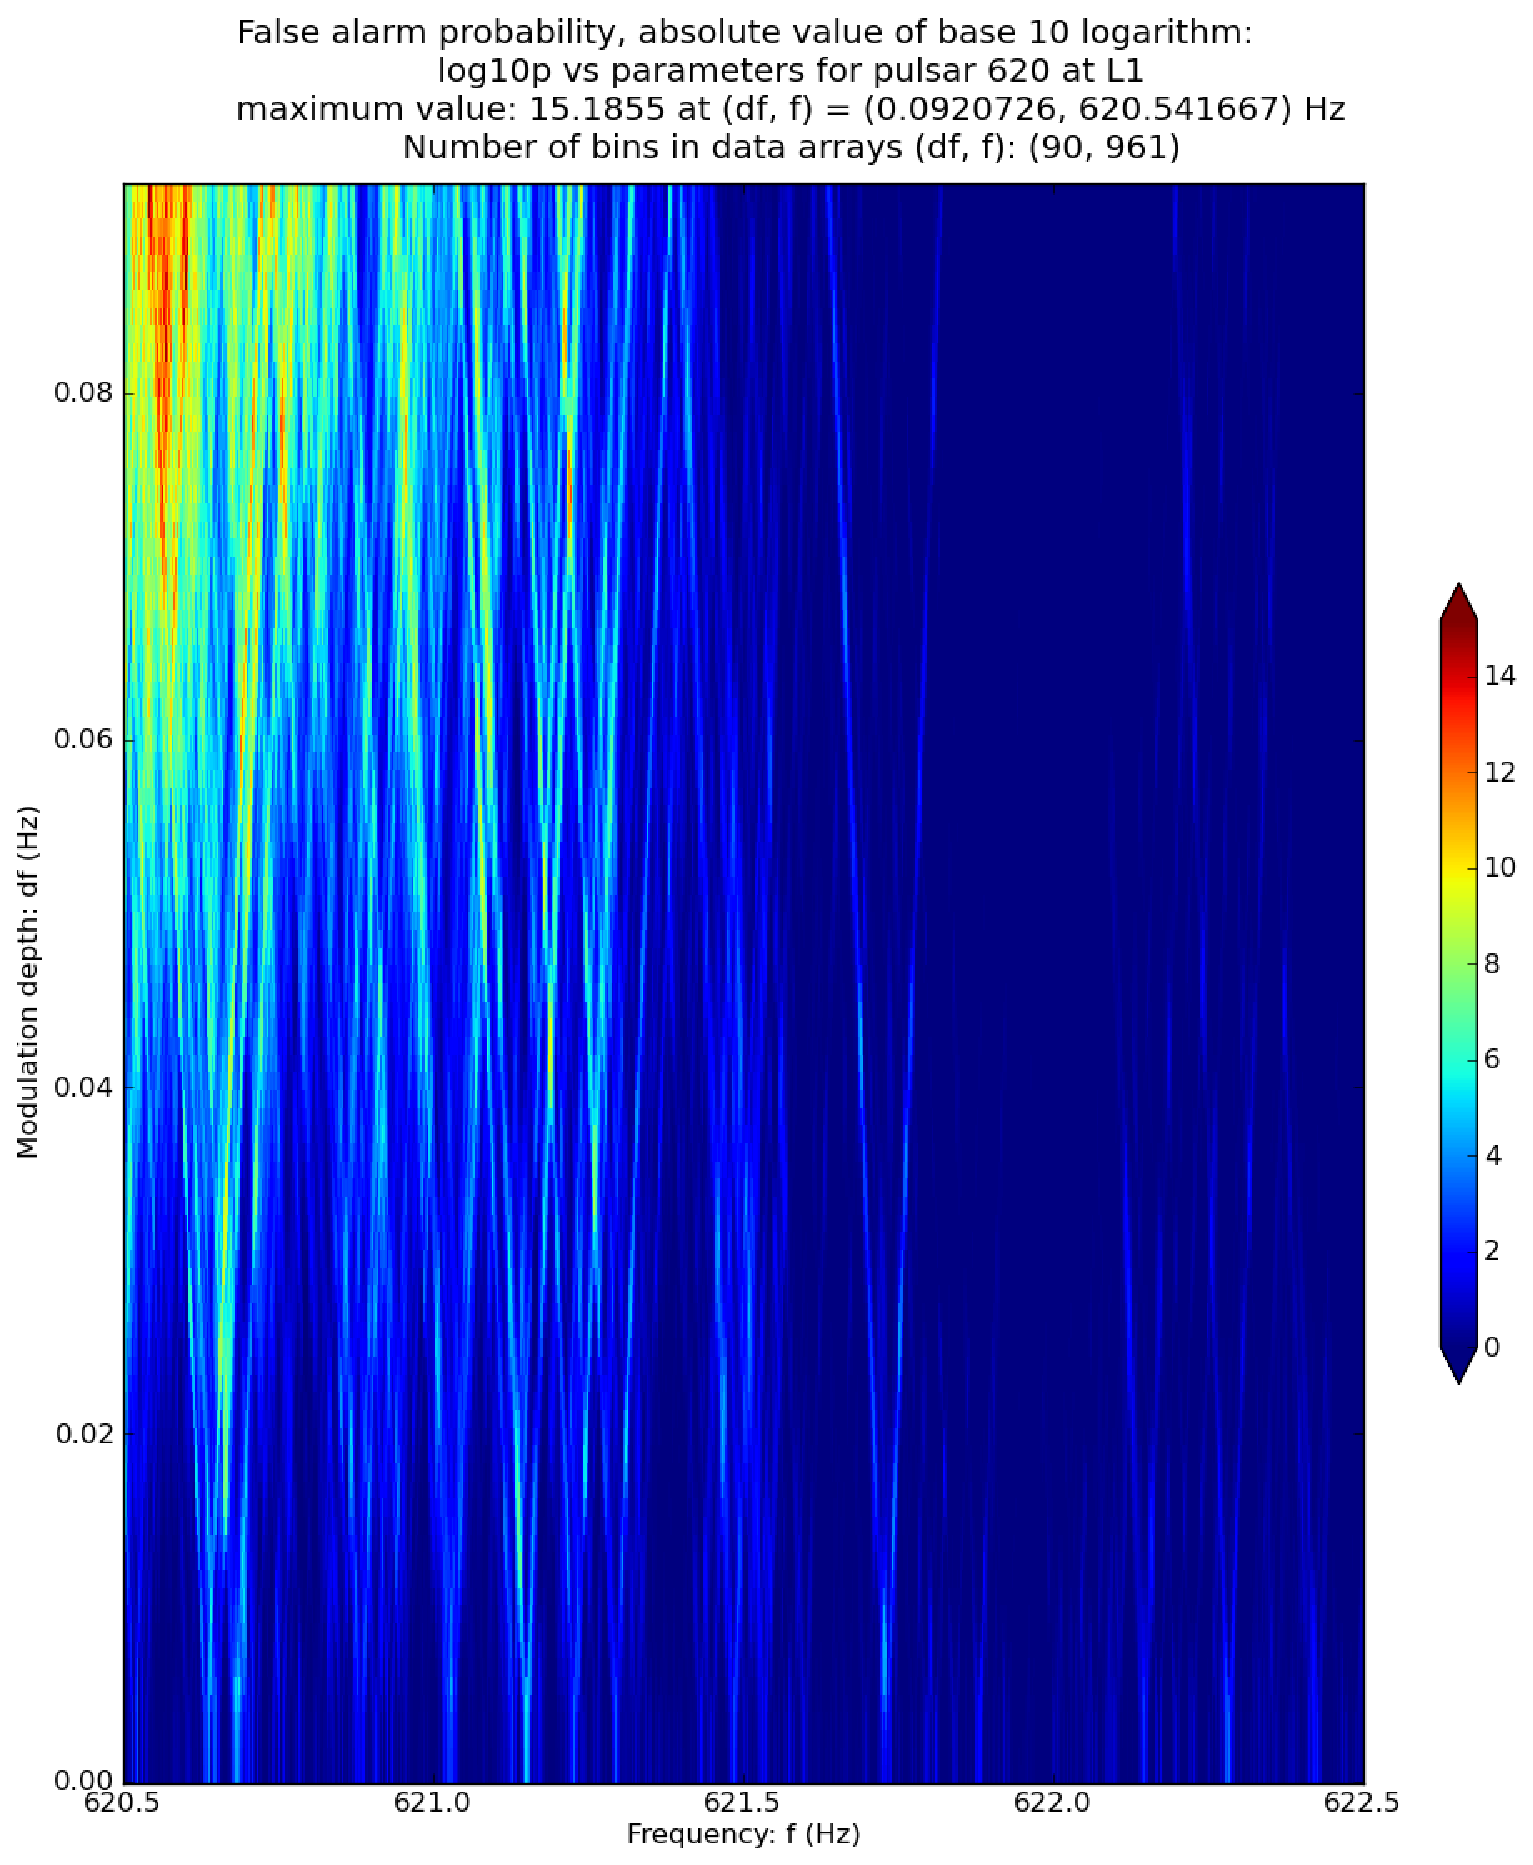
\includegraphics[width=0.4\paperwidth,height=0.2\paperheight]{plots/DFvsFresultsProb-L1_pulsar-620.eps}
\caption{
Quick look at J1751-305, L1 log10p, 621 Hz $r$-mode}
\end{center}
\end{figure}


\section{Summary of Directed TwoSpect S6 searches}

\textbf{2 kHz, $\pm 3 \sigma_{a \sin i}$ search over all S6 data from H1 \& L1}
\begin{itemize}
\item Analyze 40 to 360 Hz with 840 s SFTs,
\item Analyze 360 to 2040 Hz with 360 s SFTs,\\
(to prevent spectral leakage)
\item Now planned: overlapping bands to verify
\item Search over 300+1700 Hz = 2.0 kHz complete on H1
\item Search over 300+1700 Hz = 2.0 kHz complete on L1
\end{itemize}


\emph{S6 search \textbf{100\% done} in 30 days, with 2 kHz per H1, L1}

\begin{enumerate}
\item Should verify overlapping bands with shorter coherence length
\item Refining upper limit methodology
\item R statistic: quiet 0.1 Hz bands need investigation
\item Detection criteria: how applicable is MDC experience?
\end{enumerate}

\emph{Random polarization} $h_0$ lower limit might be $< 1.3\times10^{-24}$
\emph{Outliers} incoming: already $\sim 22$ coincident features in [40, 360] Hz

Plans for O1, first aLIGO run


\textit{As previously noted, results from this chapter are preliminary and have not been reviewed yet by the LIGO Scientific Collaboration.}

        %---------------------------------

	%The following is an example of using the commands \textit{ref}
	%and \textit{label}. With these commands theorems, chapters,
	%sections and figurres can be labeld with names in the tex file
	%and then refered to by these names in later tex files. In
	%chapter~\ref{intro} we saw section~\ref{sample_section} or
	%theorem~\ref{sample_theorem}.

	%Lastly, here is how to include a figure. First generate an
	%encapsulated postscript file in xfig, adobe illustrator or
	%some other program. The specific commands are found in
	%\textit{chap2.tex}.

        %\begin{figure}[htb]
        %\centerline{ \epsfig{figure=sample.eps, 
        %height =  1.5 in}}
        %\caption{Sample Figure}
        %\label{sample_figure}
        %\end{figure}

